  \graphicspath{ {Figs/Chapter3/} }
 \chapter{Proceso de Creación de un Modelo de red Blockchain}
 
En el presente capítulo, se describe el proceso de creación de un modelo de red \textit{blockchain} utilizando la tecnología Hyperledger IBM, específicamente Hyperledger Composer. Primeramente, se explica la elección de la tecnología; a continuación se presentan conceptos y elementos fundamentales del Hyperledger Composer y finalmente se detallan los pasos necesarios para la creación del modelo de red, siguiendo los lineamientos y conceptos de la tecnología.


\section{Selección de tecnología}
Dado los objetivos planteados en el presente proyecto y haciendo referencia al Capitulo 2, en la Sección 2.4, donde se detallan y comparan las tecnologías existentes, se sugiere el uso  de un \textit{blockchain} de tipo \textbf{privado}, pues éste se adapta mejor a los requerimientos y las necesidades establecidas por la Universidad Simón Bolívar, las cuales ameritan un mayor control sobre el acceso a recursos, roles y permisología asociada a procesos internos de la universidad. Resulta fundamental resaltar que \textit{Hyperledger Fabric} está específicamente diseñado para atender este tipo de escenarios de manera efectiva haciendo uso de su modularidad para adaptarse a los distintos escenarios dentro de las organizaciones. 

\section{Hyperledger Composer y el Modelo de Red Blockchain}

\textit{Hyperledger Composer} es un conjunto de herramientas de colaboración cuya finalidad es construir redes de negocio en \textit{blockchain} y generalmente es utilizado en conjunción de \textit{Hyperledger Fabric}. El Composer permite a los desarrolladores, mediante su abstracción centrada en el negocio, crear contratos inteligentes y aplicaciones \textit{blockchain} de forma rápida y sencilla con la finalidad de dar soluciones robustas a los diferentes problemas sin tener la preocupación inicial del despliegue e instalación de la red \textit{blockchain} a utilizar. Al estar desarrollado con JavaScript, aprovecha las herramientas y librerías modernas, como por ejemplo, node.js, npm y CLI.  

En \textit{Hyperledger Composer}, un modelo de red \textit{blockchain} hace referencia al conjunto de definiciones de los recursos, participantes, elementos y servicios necesarios  dentro de la misma. El modelo de red define el modelo de negocios, la lógica de transacciones (contratos inteligentes) y a su vez delimita las reglas de acceso y permiso lógicas~\cite{dhillon2017hyperledger}.  Dicho modelo de red, está definido en un archivo conocido como \textit{BNA} (por sus siglas en inglés {\it Bussines Network Archive}) y posee la misma extensión para denotarlo (ejemplo, \textit{<nombrearchivo>.bna}). Este archivo es crucial para poder desplegar o instalar una red en \textit{Hyperledger Fabric}. Los elementos específicos del modelo de red \textit{blockchain}, se expondrán en una sección siguiente del presente capítulo.

\section{Proceso de diseño y creación}

El proceso utilizado en la creación de un modelo de red desarrollado en \textit{Hyperledger Composer}, puede ser dividido en 3 fases: planteamiento del problema, diseño del modelo de red e implementación del mismo.

\subsection{Planteamiento del problema y requerimientos} 
Resulta fundamental entender y definir el problema de negocio que requiere solución para posteriormente establecer los requerimientos y necesidades relacionados. 

En \textit{Hyperledger Composer } se definen los siguientes recursos que hacen parte de cualquier modelo de red \textit{blockchain}:
\begin{itemize}
\item Activos: son bienes tangibles o intangibles, servicios o propiedades.
\item Participantes: son miembros de una red de negocios. Éstos pueden poseer activos y enviar transacciones. Cada participante debe contar con un identificador y puede tener otras propiedades asociadas.
\item Transacciones: mecanismo por el cual los participantes interactúan con los activos; también se les conoce como contratos inteligentes o chaincode (en el caso de \textit{Hyperledger}).
\item Reglas y Roles: ésta es la característica principal de cualquier \textit{blockchain} de negocios. Al usar las reglas y roles de acceso, se puede definir quién puede hacer qué y sobre cuáles recursos dentro de la red.
\end{itemize}


\subsection{Diseño y modelado} 
En esta fase se utilizaron una serie de elementos gráficos con la finalidad de representar los distintos recursos de la red previamente definidos. En este fase puede resultar útil la realización de modelos relacionales, diagramas de flujo, actividad, clases o BMPN; en general, cualquier representación que ayude a definir de manera clara las diferentes  interacciones entre los recursos de la red.


\subsection{Implementación y desarrollo}
Desde el punto de vista de desarrollo, el modelo de red \textit{blockchain} está conformado por 3 componentes esenciales:

\textbf{El lenguaje de modelado CTO}: el Composer posee su propio lenguaje de modelado que es utilizado para definir los activos, participantes y transacciones. Estos recursos se definen en un archivo con extensión \textit{.cto} (en honor al  proyecto original denominado \textit{Concert}~\cite{ibmDevWorks}).

Todos los recursos de este archivo están asociados a un \textit{namespace}, el cual funciona como contenedor abstracto base de todas las definiciones de clase comprendidas en la red de negocio. El \textit{namespace} está definido al comienzo del archivo \textit{.cto} de la siguiente manera:

\begin{lstlisting}
namespace org.example.basic
\end{lstlisting}

A continuación se presentan fragmentos de código para cada recurso definido con fines ilustrativos:

\textit{Activo}
\begin{lstlisting}
asset SampleAsset identified by assetId {
  o String assetId
  --> SampleParticipant owner
  o String value
}
\end{lstlisting}
Los activos se diferencian en el lenguaje \textit{CTO} con la palabra \textit{asset} al inicio de su definición y deben poseer al menos un atributo identificador como se observa en el fragmento anterior.

\textit{Participante}
\begin{lstlisting}
participant SampleParticipant identified by participantId {
  o String participantId
  o String firstName
  o String lastName
}
\end{lstlisting}
Los participantes se diferencian en el lenguaje \textit{CTO} con la palabra \textit{participant} al inicio de su definición y deben poseer al menos un atributo identificador como se observa en el fragmento.

\textit{Transaccion}
\begin{lstlisting}
transaction SampleTransaction {
  --> SampleAsset asset
  o String newValue
}
\end{lstlisting}
Las transacciones se diferencian en el lenguaje \textit{CTO} con la palabra \textit{transaction} al inicio de su definición. Pueden tener atributos pero  éstos no son obligatorios.

La letra \textbf{o} sirve para indicar un atributo del recurso, seguido de su tipo y nombre.

El símbolo \textbf{-->} indica la relación con un recurso, seguido del nombre del recurso asociado y su tipo. Esta relaciones son unilaterales.

\textbf{Chaincode o contratos inteligentes}: la lógica de las transacciones definidas en el archivo CTO se implementa gracias a este componente, utilizando el lenguaje de programación Javascript y por consecuencia se encuentran en archivos con extensión \textit{.js} dentro del Composer. A continuación se presenta la implementación lógica de la transacción \textit{SampleTransaction} expuesta en el ejemplo anterior.

\textit{sample.js}
\begin{lstlisting}
/**
 * Sample transaction processor function.
 * @param {org.example.basic.SampleTransaction} tx The sample transaction instance.
 * @transaction
 */
async function sampleTransaction(tx) { 

    // Guarda el valor anterior del activo.
    const oldValue = tx.asset.value;

    // Actualiza el activo con un nuevo valor
    tx.asset.value = tx.newValue;

    // Solicita el registro del activo.
    const assetRegistry = await getAssetRegistry('org.example.basic.SampleAsset');
    // Actualiza el activo en los registros de activos
    await assetRegistry.update(tx.asset);
}
\end{lstlisting}
La siguiente transacción realiza una actualización simple de valor en el activo \textit{SampleAsset} utilizado en los ejemplos del lenguaje de modelado.

Es importante destacar que todas las funciones \textit{.js} deben llevar la cabecera comentada, como se aprecia en el ejemplo, puesto que ésta permite enlazar las funciones lógicas con las transacciones descritas en el modelo CTO.

\textbf{Lista de Control de Accesos}: tanto el control de acceso como la permisología se rigen por un archivo llamado \textit{permissions.acl} (ACL por sus siglas en inglés {\it Access Control Language}). El archivo ACL contiene reglas que le permiten regular el acceso a los recursos de la aplicación \textit{blockchain}. Dichas reglas pueden ser definidas sobre cualquier recurso de la red, es decir, sobre transacciones, activos y participantes. La gramática utilizada para definir estas reglas se puede apreciar en el siguiente ejemplo:

\begin{lstlisting}
rule reglaSimple {
    description: "Descripcion de la regla ACL"
    participant: "org.example.SampleParticipant"
    operation: CREATE, UPDATE
    resource: "org.example.SampleAsset"
    action: ALLOW
}
\end{lstlisting}
\begin{itemize}
    \item El campo \textit{description} es utilizado para colocar una breve descripción del propósito de la regla.
    \item El campo \textit{participant} define la persona o entidad que ha enviado una transacción para su procesamiento. El valor especial \textit{ANY} puede usarse para indicar que no se aplica la comprobación de tipo de participante en la regla.
    \item  El campo \textit{operation} identifica el tipo de operación que rige la regla: \textit{CREATE}, \textit{READ}, \textit{UPDATE}. Adicionalmente, se puede utilizar \textit{ALL} para especificar que la regla rige todas las operaciones compatibles. Alternativamente, es posible utilizar usar una lista separada por comas para especificar que la regla rige un conjunto de operaciones.
    \item  El campo \textit{resource} permite definir cualquier recurso sobre el cual la regla será aplicada.
    \item  El campo \textit{action} identifica la acción de la regla, el cual puede ser \textit{ALLOW} (permitir operaciones asociadas) o \textit{DENY} (denegar operaciones asociadas).
\end{itemize}
 
Una vez desarrollados estos componentes, \textit{Hyperledger Composer} se vale de alguno  de los métodos siguientes para interactuar y probar el modelo de red desarrollado.
\begin{itemize}
    \item El primero, utiliza la herramienta \textbf{Hyperledger Composer Playground} o simplemente \textit{Playground}, que proporciona una interfaz gráfica de usuario para la configuración, implementación y prueba del modelo de red. \textit{Playground} necesita únicamente de un explorador web para empezar a crear, ejecutar y verificar los distintos recursos requeridos en la red de {\it blockchain}.
    
    \item El segundo, a través de una red real desplegada en  \textbf{Hyperledger Fabric} de forma local o en la nube. Este método es de mayor complejidad que el método anterior, ya que requiere una cantidad mayor de herramientas y configuraciones que escapan del alcance de este proyecto. La Figura~\ref{fig: composer-bna} muestra un diagrama explicativo de los componentes del \textit{Composer} y su integracion con \texit{Fabric}.
\end{itemize}

\begin{figure}[h]
\centering
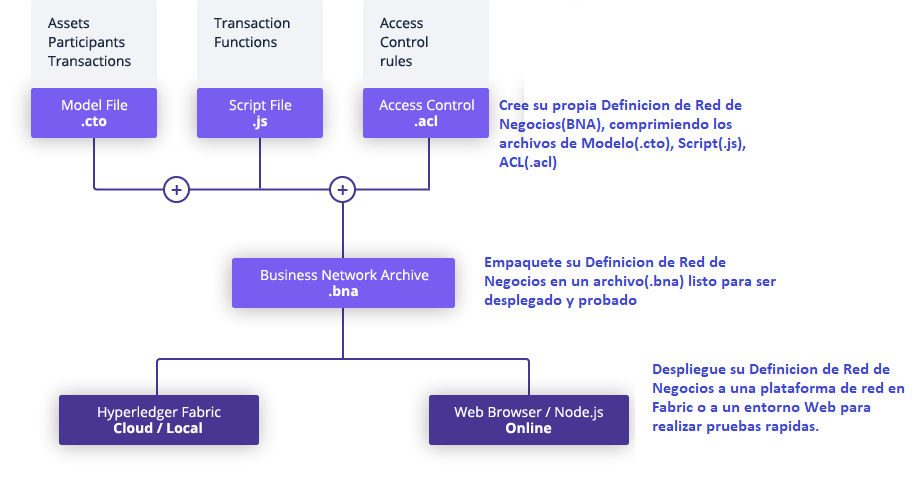
\includegraphics[width=1\textwidth]{composer-playground.png}
\caption[Fabric and Composer]{Diagrama explicativo de componentes del \textit Composer.}
\label{fig: composer-bna}
\end{figure}

